\section{使用模板}

\begin{frame}[fragile]
\frametitle{模板}
\begin{itemize}
  \item<+-> 是什么?

    \begin{itemize}
      \item 设计好的格式框架
      \item 专注于内容:\alert{不必追求与期刊排版完全一致}
      \item Word 中的样式:「学好 \LaTeX{} 可以更科学地使用 Word」
    \end{itemize}

  \item<+-> 有哪些?

    \begin{itemize}
      \item 期刊:\pkg{revtex}、\pkg{elsarticle}、\pkg{IEEEtran}……
      \item 学位论文:\pkg{thuthesis}、\pkg{ustcthesis}、\pkg{SJTUThesis}……
    \end{itemize}

  \item<+-> 怎么用?

    \begin{itemize}
      \item |\documentclass{...}|,配置参数,照常编写
      \item 可能与 \LaTeX{} 通常用法不同:\alert{看文档,看文档,看文档}
    \end{itemize}

  \item<+-> 去哪里找?

    \begin{itemize}
      \item CTAN \link{https://ctan.org} 或 GitHub \href{https://github.com}{\faGithub}
      \item 期刊官网
      \item 「湿兄用 U 盘 or 微信传给你的模板几乎一定是过时的」
    \end{itemize}
\end{itemize}
\end{frame}

\begin{frame}[fragile]
\frametitle{\pkg{revtex}}
\begin{itemize}
  \item<+-> 获取

    \begin{itemize}
      \item APS 官网 \link{https://journals.aps.org/revtex}
      \item \TeX{} Live 自带(注意检查版本)
      \item 阅读文档:|texdoc aps|
    \end{itemize}

  \item<+-> 写作

    \begin{itemize}
      \item |\documentclass[aps,prl,twocolumn,...]{revtex4-2}|
      \item 作者信息:|\title|、|\author| 等需放在 |\begin{document}| 之后
      \item 跨栏长公式:|widetext| 环境
      \item 文献引用:|\cite| + |\bibliography|,无需 |\bibliographystyle|
    \end{itemize}

  \item<+-> 编译

    \begin{itemize}
      \item 推荐 \pdfLaTeX{},也可 |latexmk -pdf|
    \end{itemize}
\end{itemize}
\end{frame}

\begin{frame}[fragile]
\frametitle{\pkg{revtex}:示例}
\setlength{\fboxsep}{0pt}
\foreach \x in {1,...,7} {%
  \fbox{\includegraphics[width=0.24\textwidth, page=\x]{examples/apssamp.pdf}}
}
\end{frame}

\begin{frame}[fragile]
\frametitle{\pkg{fduthesis}:安装}
\begin{columns}
\begin{column}{0.7\textwidth}
  \begin{itemize}
    \item<+-> 最新版本:v0.8-dev
    \item<+-> 建议直接从 GitHub 下载 \link{https://github.com/stone-zeng/fduthesis}

      \begin{itemize}
        \item Code > Download ZIP
        \item 或使用 |git clone| / |gh repo clone|
        \item 执行 |install-win.bat| 或 |install-linux.sh|,所需文件会在 |thesis| 文件夹中生成
        \item Releases 中的版本较旧
      \end{itemize}

    \item<+-> \TeX{} Live 和 Overleaf
      \link{https://www.overleaf.com/latex/templates/fduthesis-latex-thesis-template-for-fudan-university/svtdhhstkmkt}
      上的也较旧

      \begin{itemize}
        \item \CJKsout{主要怪我懒}
        \item 会尽快更新的(
      \end{itemize}
  \end{itemize}
\end{column}
\begin{column}{0.26\textwidth}
  \onslide<2->
  \includegraphics[width=\textwidth]{images/github-download.png}
\end{column}
\end{columns}
\end{frame}

\begin{frame}[fragile]
\frametitle{\pkg{fduthesis}:使用}
\begin{itemize}
  \item<+-> 文档类选项

    \begin{itemize}
      \item 论文类型:\lstinline[style=style@inline]+type = doctor|master|bachelor+
      \item 单双面模式:|oneside| 或 |twoside|
    \end{itemize}

  \item<+-> 参数设置举例

    \begin{texcode}[gobble=4, basicstyle=\scriptsize\ttfamily, moretexcs={\fdusetup},
        emph={[1]style,info,font-size,bib-resource,title,author}, alsoletter={-}]
      \fdusetup{
        style = {font-size = 5, bib-resource = {ref.bib}},
        info/title = {论动体的电动力学},
        info/author = {阿尔伯特・爱因斯坦},
      }
    \end{texcode}

  \item<+-> 文献引用

    \begin{itemize}
      \item |\cite|、|\citet|、|\parencite| 等
      \item 文献列表:|\printbibliography|
    \end{itemize}

  \item<+-> 编译

    \begin{itemize}
      \item 推荐 \XeLaTeX{},也可 |latexmk -pdfxe|
    \end{itemize}

\end{itemize}
\end{frame}

\begin{frame}[fragile]
\frametitle{\pkg{fduthesis}:示例}
\setlength{\fboxsep}{0pt}
\foreach \x in {1,...,8} {%
  \fbox{\includegraphics[width=0.24\textwidth, page=\x]{examples/fduthesis/fduthesis-template.pdf}}
}
\vspace{-0.8cm}
\end{frame}
